\documentclass[10pt]{article}
\usepackage{starlight}          % or \usepackage[letter]{starlight}
\renewcommand{\headertext}{Math \& CS Notes}

\title{Starlight Notes}
\author{Every box, macro and code block in starlight.sty}
\date{Fall 2026}

\begin{document}
\maketitle

\section{Sets and functions}

A function $f\colon A \to B$ is \term{injective} if $f(a) = f(a')$ implies $a = a'$,
and \term{surjective} if every $b \in B$ has a preimage. Throughout, $\N = \set{0, 1, 2, \dots}$.

\begin{definition}[Bijection]\label{def:bij}
  A function is a \term{bijection} if it is both injective and surjective. Equivalently,
  it has a two-sided inverse $f\inv$ with $f\inv \circ f = \id_A$ and $f \circ f\inv = \id_B$.
\end{definition}

\begin{theorem}[Cantor]\label{thm:cantor}
  For any set $A$ there is no surjection $A \to \mathcal{P}(A)$. In particular
  $\abs{A} < \abs{\mathcal{P}(A)}$.
\end{theorem}

\begin{proof}
  Suppose $f\colon A \to \mathcal{P}(A)$ is onto and let $D = \setof{a \in A}{a \notin f(a)}$.
  Then $D = f(d)$ for some $d$, and $d \in D \iff d \notin f(d) = D$, a contradiction.
\end{proof}

\begin{lemma}
  If $g \circ f$ is injective then $f$ is injective.
\end{lemma}
\begin{corollary}
  By \hyperref[thm:cantor]{Theorem~\ref*{thm:cantor}}, $\R$ is uncountable, since $\abs{\R} = \abs{\mathcal{P}(\N)}$.
\end{corollary}

\begin{example}[A bijection $\N \to \Z$]
  $f(n) = \frac{n}{2}$ for even $n$ and $f(n) = -\frac{n+1}{2}$ for odd $n$ lists
  $0, -1, 1, -2, 2, \dots$, hitting every integer exactly once.
\end{example}

\begin{remark}
  Definition~\ref{def:bij} makes no mention of cardinality; that comes later.
\end{remark}

\section{Analysis}

\begin{definition}[Limit]
  $\lim_{x \to a} f(x) = L$ if for every $\eps > 0$ there is $\delta > 0$ with
  $0 < \abs{x - a} < \delta \implies \abs{f(x) - L} < \eps$.
\end{definition}

\begin{proposition}[Integration by parts]
  \[ \int_a^b u \dd v = \Big[uv\Big]_a^b - \int_a^b v \dd u,
     \qquad \deriv{}{x}\paren*{\int_a^x f(t) \dd t} = f(x). \]
\end{proposition}

\begin{problem}[Series]\label{prob:series}
  Evaluate $\displaystyle\sum_{n=1}^{\infty} \frac{1}{n(n+1)}$ and decide whether
  $\sum_n \frac{1}{n \log n}$ converges.
\end{problem}
\begin{solution}
  Telescoping, $\frac{1}{n(n+1)} = \frac1n - \frac1{n+1}$, so the partial sums are $1 - \frac1{N+1}$
  and the series equals \ans{1}. The second diverges by the integral test:
  $\int_2^\infty \frac{\dd x}{x \log x} = \big[\log\log x\big]_2^\infty = \infty$.
\end{solution}

\begin{warning}
  $\sum a_n$ converging does not follow from $a_n \to 0$; the harmonic series is the standard counterexample.
\end{warning}

\subsection{Linear algebra}
For $A \in \R^{m \times n}$, $\rank A + \dim\ker A = n$, and $\norm{Ax}_2 \le \norm{A}\norm{x}_2$.
\[
  A = \begin{pmatrix} 2 & 1 \\ 1 & 2 \end{pmatrix}, \quad
  A\T = A, \quad \tr A = 4, \quad \det A = 3, \quad
  \inner{Ax}{x} = 2x_1^2 + 2x_1x_2 + 2x_2^2 > 0 .
\]

\begin{tip}
  To check a matrix is positive definite, all its leading principal minors being positive is quickest by hand.
\end{tip}

\section{Algorithms}

\begin{theorem*}[Master theorem, case 2]
  If $T(n) = aT(n/b) + \bigT{n^{\log_b a}}$ then $T(n) = \bigT{n^{\log_b a}\log n}$.
\end{theorem*}

\begin{pseudo}{Binary search}
  \begin{algorithmic}[1]
    \Require sorted array $A[1..n]$, target $x$
    \State $lo \gets 1$, $hi \gets n$
    \While{$lo \le hi$}
      \State $mid \gets \floor{(lo + hi)/2}$ \Comment{never overflows in maths}
      \If{$A[mid] = x$} \Return $mid$
      \ElsIf{$A[mid] < x$} $lo \gets mid + 1$
      \Else\ $hi \gets mid - 1$
      \EndIf
    \EndWhile
    \State \Return \textsc{not found}
  \end{algorithmic}
\end{pseudo}

Each iteration halves $hi - lo$, so it runs in $\bigO{\log n}$ time; the \CC{} version uses
\code|std::lower_bound| for the same thing.

\begin{codeblock}{search.cpp}
#include <vector>
// returns the index of x in a, or -1
int search(const std::vector<int>& a, int x) {
    int lo = 0, hi = static_cast<int>(a.size()) - 1;
    while (lo <= hi) {
        int mid = lo + (hi - lo) / 2;      // no overflow
        if (a[mid] == x) return mid;
        if (a[mid] < x) lo = mid + 1; else hi = mid - 1;
    }
    return -1;
}
\end{codeblock}

\begin{codeblock}[lang=Python]{search.py}
def search(a: list[int], x: int) -> int:
    """Binary search; returns -1 if x is missing."""
    lo, hi = 0, len(a) - 1
    while lo <= hi:
        mid = (lo + hi) // 2
        if a[mid] == x:
            return mid
        lo, hi = (mid + 1, hi) if a[mid] < x else (lo, mid - 1)
    return -1
\end{codeblock}

\begin{terminal}
$ g++ -std=c++20 -O2 search.cpp -o search && ./search
found 42 at index 17
\end{terminal}

\subsection{Graphs and plots}
\begin{minipage}[t]{0.47\linewidth}
  \centering
  \begin{tikzpicture}[node distance=9mm and 11mm]
    \node[vertex] (a) {$a$};
    \node[vertex, right=of a] (b) {$b$};
    \node[vertex, below=of a] (c) {$c$};
    \node[vertex, hot, right=of c] (d) {$d$};
    \draw[arrow] (a) -- node[above, font=\scriptsize] {3} (b);
    \draw[arrow] (a) -- node[left, font=\scriptsize] {1} (c);
    \draw[arrow] (c) -- node[below, font=\scriptsize] {2} (d);
    \draw[arrow] (b) -- node[right, font=\scriptsize] {4} (d);
  \end{tikzpicture}
  \par\smallskip{\small Shortest $a \to d$ path: $a, c, d$ (cost 3).}
\end{minipage}\hfill
\begin{minipage}[t]{0.5\linewidth}
  \centering
  \begin{tikzpicture}
    \begin{axis}[width=\linewidth, height=4.2cm, xmin=1, xmax=64, ymin=0, ymax=64,
                 xlabel={$n$}, legend pos=north west]
      \addplot+[no marks, domain=1:64, samples=60] {x};
      \addplot+[no marks, domain=1:64, samples=60] {x*ln(x)/ln(2)/6};
      \addplot+[no marks, domain=1:64, samples=60] {ln(x)/ln(2)};
      \legend{$n$, $\tfrac16 n\lg n$, $\lg n$}
    \end{axis}
  \end{tikzpicture}
\end{minipage}

\begin{center}
  \begin{tikzcd}[column sep=large]
    A \arrow[r, "f"] \arrow[dr, "g \circ f"'] & B \arrow[d, "g"] \\ & C
  \end{tikzcd}
  \qquad
  \begin{tabular}{lcc}
    \toprule
    \thead{Structure} & \thead{Search} & \thead{Insert} \\
    \midrule
    Sorted array  & $\bigO{\log n}$ & $\bigO{n}$ \\
    Balanced BST  & $\bigO{\log n}$ & $\bigO{\log n}$ \\
    Hash table    & $\bigO{1}$ avg. & $\bigO{1}$ avg. \\
    \bottomrule
  \end{tabular}
\end{center}

\subsection{Probability}
For independent $X, Y$: $\E[X + Y] = \E X + \E Y$, $\Var(X + Y) = \Var X + \Var Y$, and
$\Prob[A \given B] = \Prob[A \cap B] / \Prob[B]$.

\begin{exercise}
  Show that a random permutation of $[n]$ has $1$ fixed point in expectation.
  \begin{enumerate}
    \item Write the count as $\sum_i X_i$ with indicators $X_i$.
    \item Use linearity: $\E X_i = \frac1n$.
  \end{enumerate}
\end{exercise}

\begin{summary}
  \begin{itemize}
    \item Cantor: $\abs{A} < \abs{\mathcal{P}(A)}$ \quad\twinkle[lilac]\quad telescoping sums \quad\twinkle[lilac]\quad binary search is $\bigO{\log n}$.
    \item \hl{Linearity of expectation needs no independence.}
  \end{itemize}
\end{summary}

\end{document}
